\documentclass[border=5pt]{standalone}
% Shared by every figure. Colour marks the TYPE of a quantity, never decoration:
%   blue   (vec) equivariant: rotates with its fragment     -- solid arrows
%   orange (inv) invariant: unchanged by any rotation        -- dashed arrows
%   aqua   (att) attention / communication between elements
%   violet (out) what the network outputs
% Text is always ink; a coloured mark next to it carries the meaning.
\usepackage{amsmath,amssymb,bm}
\usepackage{tikz}
\usetikzlibrary{arrows.meta,positioning,fit,backgrounds,calc,shapes.geometric,
  shapes.misc,decorations.pathreplacing,decorations.pathmorphing,matrix,
  patterns,cd,shadows}
\definecolor{vec}{HTML}{2A78D6}
\definecolor{inv}{HTML}{EB6834}
\definecolor{att}{HTML}{1BAF7A}
\definecolor{out}{HTML}{4A3AA7}
\definecolor{ink}{HTML}{0B0B0B}
\definecolor{ink2}{HTML}{52514E}
\definecolor{ink3}{HTML}{8A877F}
\definecolor{neutral}{HTML}{F0EFEC}
\definecolor{rule}{HTML}{CFCCC4}
\definecolor{pieceA}{HTML}{E4E1DA}
\definecolor{pieceB}{HTML}{CDC9BF}
\definecolor{pieceC}{HTML}{B3AEA2}
\colorlet{vecfill}{vec!9}
\colorlet{invfill}{inv!10}
\colorlet{attfill}{att!11}
\colorlet{outfill}{out!9}
\tikzset{
  >={Stealth[length=2.3mm,width=1.7mm]},
  every picture/.style={line cap=round, line join=round},
  box/.style={draw=ink2, fill=neutral, rounded corners=2.5pt, align=center,
    font=\small, inner sep=4pt, minimum height=8mm, text=ink, line width=0.6pt, nohyph},
  vecbox/.style={box, draw=vec, fill=vecfill},
  invbox/.style={box, draw=inv, fill=invfill},
  attbox/.style={box, draw=att, fill=attfill},
  outbox/.style={box, draw=out, fill=outfill},
  plain/.style={box, draw=ink3, fill=white},
  arr/.style={->, draw=ink2, line width=0.7pt},
  vecarr/.style={->, draw=vec, line width=1.1pt},
  invarr/.style={->, draw=inv, line width=1.1pt, dash pattern=on 3.2pt off 1.8pt},
  attarr/.style={->, draw=att, line width=1.1pt, dash pattern=on 1.2pt off 1.4pt},
  outarr/.style={->, draw=out, line width=1.1pt},
  nohyph/.style={execute at begin node={\hyphenpenalty=10000\exhyphenpenalty=10000\relax}},
  lbl/.style={font=\footnotesize, text=ink2, align=center, nohyph},
  tlbl/.style={font=\footnotesize, text=ink, align=center, nohyph},
  group/.style={draw=ink3, dashed, rounded corners=5pt, inner sep=7pt},
  op/.style={circle, draw=ink2, fill=white, inner sep=0pt, minimum size=5.2mm,
    font=\small, line width=0.6pt},
  piece/.style={fill=#1, draw=none},
  intact/.style={draw=ink2, line width=0.6pt},
  fracture/.style={draw=ink, line width=1.5pt},
  token/.style={circle, fill=att, draw=white, line width=0.5pt, inner sep=0pt,
    minimum size=4.2pt},
  vtx/.style={circle, fill=ink, inner sep=0pt, minimum size=3pt},
  panel/.style={font=\small\bfseries, text=ink, anchor=north west},
}
% one piece of the cartoon, in its own centred frame: fill, intact edge, fracture edge
\newcommand{\drawpiece}[2]{% #1 = A|B|C, #2 = fill colour
  \fill[#2] \csname Piece#1\endcsname;
  \draw[intact] \csname Intact#1\endcsname;
  \draw[fracture] \csname Crack#1\endcsname;}
% a legend entry: a short line in a given style, then its text
\newcommand{\legendline}[3]{% #1 position, #2 style, #3 text
  \draw[#2] (#1) -- ++(0.7,0) node[right, tlbl, text=ink] {#3};}

\begin{document}
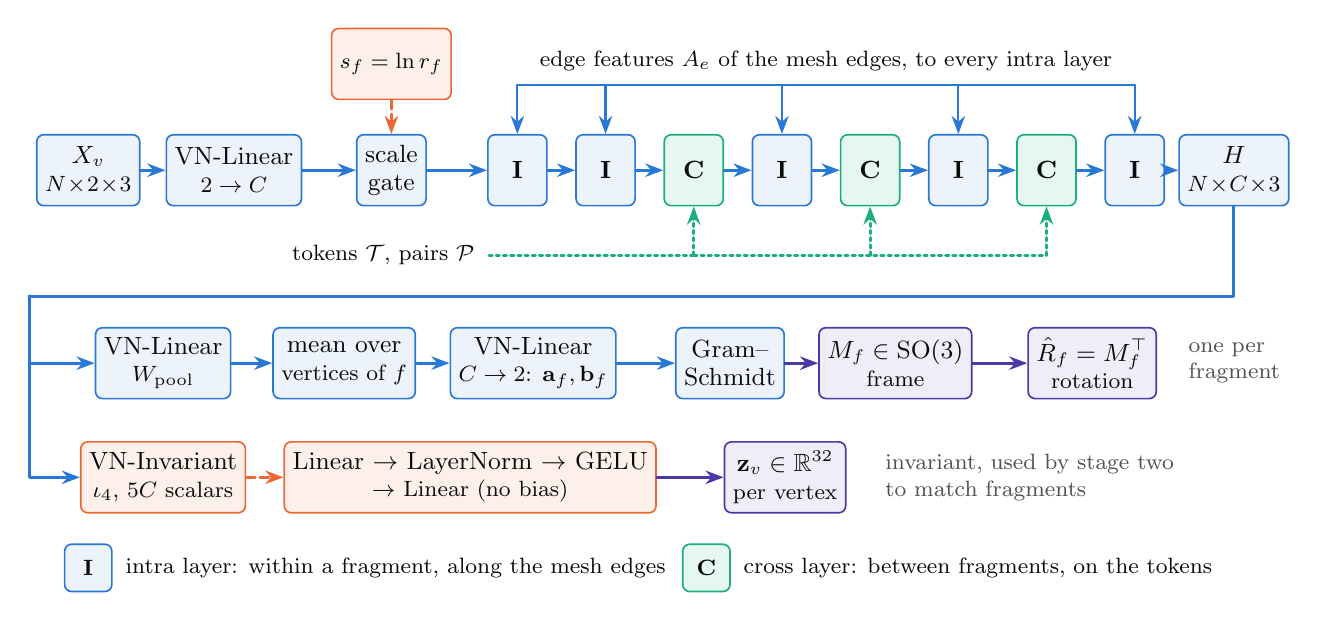
\begin{tikzpicture}
  \tikzset{
    sb/.style={font=\small, minimum height=9mm, inner sep=3pt},
    layer/.style={vecbox, font=\small\bfseries, minimum width=7.5mm, minimum height=9mm, inner sep=1pt},
    xlayer/.style={layer, draw=att, fill=attfill},
  }
  % ---------------- backbone row ----------------
  \node[vecbox, sb, align=center] (x) at (0,0) {$X_v$\\[-1pt] {\footnotesize $N\!\times\!2\!\times\!3$}};
  \node[vecbox, sb, align=center] (emb) at (1.85,0) {VN-Linear\\[-1pt] {\footnotesize $2\to C$}};
  \node[vecbox, sb, align=center] (gate) at (3.85,0) {scale\\[-1pt] gate};
  \node[invbox, sb, font=\footnotesize] (lr) at (3.85,1.35) {$s_f=\ln r_f$};
  \draw[vecarr] (x) -- (emb);
  \draw[vecarr] (emb) -- (gate);
  \draw[invarr] (lr) -- (gate);
  \def\kinds{I/intra/0,I/intra/1,C/cross/2,I/intra/3,C/cross/4,I/intra/5,C/cross/6,I/intra/7}
  \foreach \t/\k/\n in \kinds{
    \pgfmathsetmacro\xx{5.45+1.12*\n}
    \ifnum\pdfstrcmp{\k}{intra}=0
      \node[layer] (L\n) at (\xx,0) {I};
    \else
      \node[xlayer] (L\n) at (\xx,0) {C};
    \fi}
  \draw[vecarr] (gate) -- (L0);
  \foreach \a/\b in {0/1,1/2,2/3,3/4,4/5,5/6,6/7}{\draw[vecarr] (L\a) -- (L\b);}
  \node[vecbox, sb, align=center] (H) at (14.55,0) {$H$\\[-1pt] {\footnotesize $N\!\times\!C\!\times\!3$}};
  \draw[vecarr] (L7) -- (H);
  % edge features feed every intra layer; tokens and pairs feed every cross layer
  \draw[vec, line width=0.8pt] (L0.north) ++(0,0.62) -- ($(L7.north)+(0,0.62)$);
  \node[tlbl, anchor=south] at ($(L3.north)!0.5!(L4.north)+(0,0.68)$) {edge features $A_e$ of the mesh edges, to every intra layer};
  \foreach \n in {0,1,3,5,7}{\draw[vecarr, line width=0.8pt] ($(L\n.north)+(0,0.62)$) -- (L\n.north);}
  \draw[att, line width=1.0pt, dash pattern=on 1.2pt off 1.4pt] (L2.south) ++(0,-0.62) -- ($(L6.south)+(0,-0.62)$);
  \draw[att, line width=1.0pt, dash pattern=on 1.2pt off 1.4pt] ($(L2.south)+(0,-0.62)$) -- ++(-2.65,0)
    node[left, tlbl] {tokens $\mathcal T$, pairs $\mathcal P$};
  \foreach \n in {2,4,6}{\draw[attarr] ($(L\n.south)+(0,-0.62)$) -- (L\n.south);}

  % ---------------- return bus to the heads ----------------
  \draw[vec, line width=1.1pt] (H.south) -- (14.55,-1.6) -- (-0.75,-1.6) coordinate (b2);
  % rotation head
  \node[vecbox, sb, align=center] (pool) at (0.95,-2.45) {VN-Linear\\[-1pt] {\footnotesize $W_{\mathrm{pool}}$}};
  \node[vecbox, sb, align=center] (mean) at (3.25,-2.45) {mean over\\[-1pt] {\footnotesize vertices of $f$}};
  \node[vecbox, sb, align=center] (head) at (5.65,-2.45) {VN-Linear\\[-1pt] {\footnotesize $C\to 2$: $\mathbf a_f,\mathbf b_f$}};
  \node[vecbox, sb, align=center] (gs) at (8.15,-2.45) {Gram--\\[-1pt] Schmidt};
  \node[outbox, sb, align=center] (M) at (10.25,-2.45) {$M_f\in\mathrm{SO}(3)$\\[-1pt] {\footnotesize frame}};
  \node[outbox, sb, align=center] (R) at (12.75,-2.45) {$\hat R_f=M_f^{\top}$\\[-1pt] {\footnotesize rotation}};
  \draw[vecarr] (b2) |- (pool.west);
  \draw[vecarr] (pool) -- (mean);
  \draw[vecarr] (mean) -- (head);
  \draw[vecarr] (head) -- (gs);
  \draw[outarr] (gs) -- (M);
  \draw[outarr] (M) -- (R);
  % embedding head
  \node[invbox, sb, align=center] (rd) at (0.95,-3.9) {VN-Invariant\\[-1pt] {\footnotesize $\iota_4$, $5C$ scalars}};
  \node[invbox, sb, align=center] (mlp) at (4.85,-3.9) {Linear $\to$ LayerNorm $\to$ GELU\\[-1pt] {\footnotesize $\to$ Linear (no bias)}};
  \node[outbox, sb, align=center] (z) at (8.85,-3.9) {$\mathbf z_v\in\mathbb R^{32}$\\[-1pt] {\footnotesize per vertex}};
  \draw[vecarr] (b2) |- (rd.west);
  \draw[invarr] (rd) -- (mlp);
  \draw[outarr] (mlp) -- (z);
  \node[lbl, anchor=west, align=left] at (10.0,-3.9) {invariant, used by stage two\\ to match fragments};
  \node[lbl, anchor=west, align=left] at (13.85,-2.45) {one per\\ fragment};

  % ---------------- legend ----------------
  \begin{scope}[shift={(0.0,-5.05)}]
    \node[layer, minimum height=6mm, minimum width=6mm, font=\footnotesize\bfseries] at (0,0) {I};
    \node[tlbl, anchor=west] at (0.35,0) {intra layer: within a fragment, along the mesh edges};
    \node[xlayer, minimum height=6mm, minimum width=6mm, font=\footnotesize\bfseries] at (7.85,0) {C};
    \node[tlbl, anchor=west] at (8.2,0) {cross layer: between fragments, on the tokens};
  \end{scope}
\end{tikzpicture}
\end{document}
